\chapter{Gasuitwisseling en saptransport bij planten}\label{ch:b1:plant-transport}

Boven in een sequoia, honderd meter boven de grond, wordt water uit de
bodem getrokken door de verdamping aan de \omterm{def:b1:flowering-plant-organization:organs}{bladeren}, omhoog door een kolom
dode \omterm{def:b1:cell-unit-of-life:cell}{cellen} die niet breder is dan een haar, onder een spanning die een
stalen draad van dezelfde doorsnede zou knappen. Er is geen pomp; het water
wordt gehesen door dezelfde \omterm{def:b1:water-small-molecules:water}{waterstofbruggen} waarmee het aan zichzelf
kleeft. Intussen stroomt in een tweede stel buizen naast het eerste de
suiker die die \omterm{def:b1:flowering-plant-organization:organs}{bladeren} hebben gemaakt de andere kant op, geduwd door een
druk die de \omterm{def:b1:flowering-plant-organization:organs}{bladeren} zelf opwekken. De twee leidingstelsels van een plant,
het \omterm{def:b1:flowering-plant-organization:tissues}{xyleem} en het \omterm{def:b1:plant-transport:phloem}{floëem}, worden gedreven door natuurkunde die de plant
opzet en daarna laat lopen. Dit hoofdstuk beschrijft de \omterm{def:b1:plant-transport:stoma}{huidmondjes}
waardoor een \omterm{def:b1:flowering-plant-organization:organs}{blad} water tegen koolstofdioxide ruilt, het
cohesie--spanningsmechanisme dat sap optilt, de \omterm{def:b1:flowering-plant-organization:tissues}{vaten} die het vervoeren,
het \omterm{thm:b1:plant-transport:pressureflow}{drukstroommechanisme} dat suiker verplaatst, en het compromis tussen
drinken en eten dat het geheel beheerst.

\section{Huidmondjes: de poort}

\begin{definition}[Huidmondje, sluitcellen]\label{def:b1:plant-transport:stoma}
\index{huidmondje}\index{sluitcel}
Een \emph{huidmondje} is een porie in de epidermis van een \omterm{def:b1:flowering-plant-organization:organs}{blad} (of een
groene \omterm{def:b1:flowering-plant-organization:organs}{stengel}), begrensd door twee \emph{sluitcellen}: niervormige \omterm{def:b1:cell-unit-of-life:cell}{cellen}
waarvan de wanden aan de kant van de porie verdikt zijn en waarvan de
cellulosemicrofibrillen er als hoepels omheen lopen. Wanneer de sluitcellen
water opnemen en zwellen, beletten de hoepels hen breder te worden en
dwingen zij hen uit elkaar te buigen: de porie gaat open. Verliezen zij
water, dan sluit zij. Een \omterm{def:b1:flowering-plant-organization:organs}{blad} draagt enkele honderden huidmondjes per
vierkante millimeter, meestal aan zijn onderkant; open beslaan hun poriën
één of twee procent van het bladoppervlak en gaat vrijwel de hele
gasuitwisseling erdoorheen.
\end{definition}

\begin{omfigure}
\begin{tikzpicture}
  \node[anchor=south west, inner sep=0] (img) at (0,0)
    {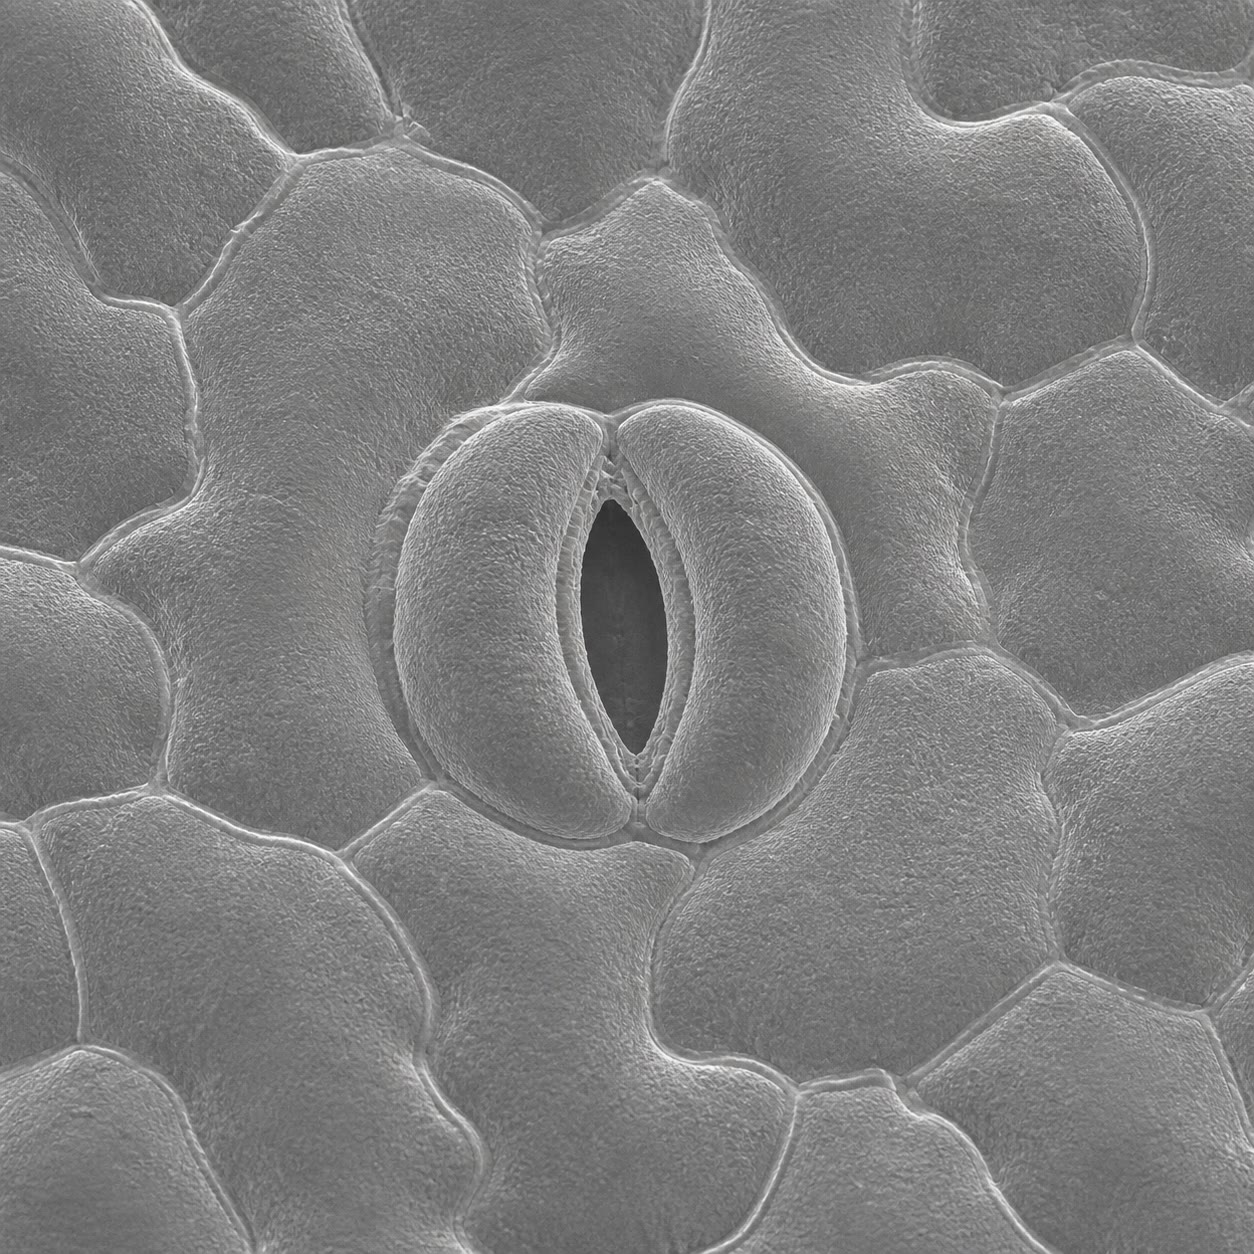
\includegraphics[width=0.4\linewidth]{images/book2/ai/g12-plant-stoma-sem.jpg}};
  \begin{scope}[x={(img.south east)}, y={(img.north west)},
      every node/.style={font=\small}]
    \draw[omDef, thick] (0.50,0.50) -- (0.50,1.08) node[above] {porie};
    \draw[omDef, thick] (0.30,0.55) -- (-0.03,0.70) node[left, align=right] {sluitcel:\\ dikke binnenwand};
    \draw[omDef, thick] (0.80,0.30) -- (1.03,0.20) node[right, align=left] {epidermiscellen\\ met cuticula};
  \end{scope}
\end{tikzpicture}

{\small Een \omterm{def:b1:plant-transport:stoma}{huidmondje} van buitenaf gezien: twee \omterm{def:b1:plant-transport:stoma}{sluitcellen} rond de porie,
gevat in een gewaste epidermis. De porie gaat open als de \omterm{def:b1:plant-transport:stoma}{sluitcellen}
zwellen.}
\end{omfigure}

\begin{proposition}[Hoe een huidmondje opengaat, en wanneer]\label{prop:b1:plant-transport:opening}
\index{abscisinezuur}
De \omterm{def:b1:plant-transport:stoma}{sluitcellen} openen de porie door protonen uit te pompen
(\cref{ch:b1:plant-water-minerals}), wat kalium en chloride naar binnen
drijft en binnenin malaat doet ontstaan; de opgeloste stoffen verlagen hun
\omterm{def:b1:membranes-transport:osmosis}{waterpotentiaal}, water volgt uit de naburige \omterm{def:b1:cell-unit-of-life:cell}{cellen}, en hun \omterm{def:b1:eukaryotic-cell:plantcell}{turgor} stijgt
met een megapascal. Het omkeren van de ionenstromen sluit de porie in
enkele minuten. De signalen: \emph{licht} (blauw licht rechtstreeks op de
\omterm{def:b1:plant-transport:stoma}{sluitcellen}, en de daling van het inwendige $\mathrm{CO_2}$ zodra de
fotosynthese begint) opent; \emph{een hoog inwendig $\mathrm{CO_2}$} sluit;
\emph{waterstress} sluit, via het hormoon \emph{\omterm{prop:b1:plant-transport:opening}{abscisinezuur}}, dat in
verwelkende \omterm{def:b1:flowering-plant-organization:organs}{wortels} en \omterm{def:b1:flowering-plant-organization:organs}{bladeren} wordt gemaakt en binnen minuten ionverlies
uit de \omterm{def:b1:plant-transport:stoma}{sluitcellen} op gang brengt; droge lucht sluit. Het \omterm{def:b1:flowering-plant-organization:organs}{blad} opent zijn
poort wanneer koolstof het water waard is en doet haar dicht wanneer water
schaars is --- en de meeste planten doen dat in een dagelijks ritme, open
bij dageraad en dicht bij schemering, dat bij aanhoudend licht dagenlang
doorloopt.
\end{proposition}

\begin{omfigure}
\begin{tikzpicture}
\begin{axis}[
  width=0.88\linewidth, height=6.0cm,
  axis x line=bottom, axis y line=left,
  xmin=0, xmax=24, ymin=0, ymax=1.15,
  xlabel={tijdstip van de dag (h)}, ylabel={relatieve waarde},
  xlabel style={font=\small, at={(axis description cs:0.5,-0.12)}, anchor=north},
  ylabel style={font=\small},
  tick label style={font=\small}, xtick={0,4,8,12,16,20,24}, ytick={0,0.5,1},
  legend style={font=\small, at={(0.5,-0.24)}, anchor=north, draw=none, legend columns=3, /tikz/every even column/.append style={column sep=0.4cm}},
  clip=false,
]
\addplot[very thick, omExo, smooth] coordinates {(0,0.05) (5,0.05) (6,0.3) (7,0.8) (8,1.0) (11,1.0) (12,0.75) (13,0.5) (14,0.55) (16,0.8) (18,0.6) (19,0.2) (20,0.05) (24,0.05)};
\addlegendentry{opening van de huidmondjes}
\addplot[very thick, omDef, smooth] coordinates {(0,0) (5,0) (6,0.1) (8,0.5) (10,0.85) (12,1.0) (14,0.9) (16,0.6) (18,0.3) (19,0.1) (20,0) (24,0)};
\addlegendentry{transpiratie}
\addplot[very thick, omThm, smooth] coordinates {(0,0.2) (5,0.2) (7,0.3) (9,0.55) (11,0.8) (13,1.0) (15,0.95) (17,0.7) (19,0.4) (21,0.25) (24,0.2)};
\addlegendentry{bladwaterpotentiaal (teken omgekeerd)}
\end{axis}
\end{tikzpicture}

{\small Een zomerdag voor een \omterm{def:b1:flowering-plant-organization:organs}{blad}. De \omterm{def:b1:plant-transport:stoma}{huidmondjes} gaan bij dageraad open,
de \omterm{thm:b1:plant-transport:cohesiontension}{transpiratie} stijgt met de zon en de droogte van de lucht, en de
\omterm{def:b1:membranes-transport:osmosis}{waterpotentiaal} van het \omterm{def:b1:flowering-plant-organization:organs}{blad} daalt terwijl de kolom onder spanning wordt
gezet; midden op de dag sluiten de \omterm{def:b1:plant-transport:stoma}{huidmondjes} zich in droge lucht deels en
herstelt het \omterm{def:b1:flowering-plant-organization:organs}{blad} zich een beetje vóór de namiddag.}
\end{omfigure}

\section{Water optillen: cohesie en spanning}

\begin{theorem}[Het cohesie--spanningsmechanisme]\label{thm:b1:plant-transport:cohesiontension}
\index{cohesie--spanningstheorie}\index{transpiratie}
Water stijgt in het \omterm{def:b1:flowering-plant-organization:tissues}{xyleem} omdat het van boven wordt \emph{getrokken}, niet
van onder geduwd. De verdamping aan de natte wanden van de mesofylcellen
van het \omterm{def:b1:flowering-plant-organization:organs}{blad} naar de luchtholten (\emph{\omterm{thm:b1:plant-transport:cohesiontension}{transpiratie}}) trekt het water in
de fijne poriën van de wand tot gekromde menisci, waarvan de
oppervlaktespanning het water erachter onder spanning zet; die spanning
wordt door de aaneengesloten waterkolommen in het \omterm{def:b1:flowering-plant-organization:tissues}{xyleem}, die door cohesie
bijeen worden gehouden (de \omterm{def:b1:water-small-molecules:water}{waterstofbruggen} van
\cref{ch:b1:water-small-molecules}), langs de \omterm{def:b1:flowering-plant-organization:organs}{stengel} omlaag tot in de
\omterm{def:b1:flowering-plant-organization:organs}{wortels} doorgegeven, en tilt water uit de bodem. Om een kolom van hoogte
$h$ tegen de zwaartekracht in te houden is een spanning $\rho g h$ nodig
--- \qty{1}{MPa} per honderd meter --- plus wat er nodig is om de wrijving
van de stroming te overwinnen, ongeveer nog eens zoveel; de kolommen van
een hoge boom staan op \qtyrange{-2}{-3}{MPa}, ruim binnen de treksterkte
van water in een fijne buis.
\end{theorem}
\begin{proof}[Bewijsmateriaal]
Dixon en Joly (1894) toonden dat water in een afgesloten glazen buis
spanningen van vele megapascals verdraagt zonder te breken, en dat een
verdampende beblaarde tak, afgesloten op een buis met water die in kwik
staat, het kwik hoger tilt dan de luchtdruk zou kunnen. De \emph{drukkamer}
van Scholander (1965) meet de spanning rechtstreeks: een afgesneden \omterm{def:b1:flowering-plant-organization:organs}{blad}
wordt in een kamer afgesloten met zijn steel naar buiten, en de gasdruk die
het sap net tot aan het snijvlak terugduwt is gelijk aan de spanning
waaronder het sap stond --- \qtyrange{0.5}{1}{MPa} in een goed bewaterd
gewas op het middaguur, \qtyrange{2}{4}{MPa} in een woestijnstruik of in de
kroon van een hoge boom. Een dendrometer laat de stam van een boom overdag
krimpen, terwijl de spanning de \omterm{def:b1:flowering-plant-organization:tissues}{vaten} samenknijpt, en 's nachts weer
zwellen; een thermometer in het hout laat zien dat het sap het snelst
stroomt wanneer de \omterm{thm:b1:plant-transport:cohesiontension}{transpiratie} het hoogst is, en 's nachts stilvalt. Er is
geen levende \omterm{def:b1:cell-unit-of-life:cell}{cel} voor nodig: een met gif of hitte gedode \omterm{def:b1:flowering-plant-organization:organs}{stengel} geleidt
nog steeds.
\end{proof}

\begin{omfigure}
\begin{tikzpicture}[font=\footnotesize, >=Stealth, line cap=round]
  % leaf at top, stem, root in soil; water potentials
  \draw[thick, omExo!70!black, fill=omExo!25] (0,7.0) .. controls (1.4,7.8) and (2.6,7.6) .. (3.0,7.0) .. controls (2.6,6.4) and (1.4,6.2) .. (0,7.0);
  \node[font=\scriptsize] at (1.5,7.0) {blad, $\Psi = \qty{-1.5}{MPa}$};
  \draw[line width=6pt, omDef!35] (1.5,6.3) -- (1.5,1.6);
  \draw[very thick, omDef!70!black] (1.38,6.3) -- (1.38,1.6) (1.62,6.3) -- (1.62,1.6);
  \node[font=\scriptsize, anchor=west, align=left] at (1.75,4.0) {xyleem: een aaneengesloten waterkolom\\ onder spanning, $\Psi = \qty{-1.0}{MPa}$ op halve hoogte};
  \fill[pattern=north east lines, pattern color=omProp!60] (-1.0,0) rectangle (4.0,1.6);
  \draw[thick, omDef!60!black] (1.5,1.6) -- (1.5,0.6) (1.5,1.3) -- (0.6,0.4) (1.5,1.0) -- (2.4,0.3);
  \node[font=\scriptsize, anchor=west] at (2.7,1.1) {wortel, $\Psi = \qty{-0.5}{MPa}$};
  \node[font=\scriptsize, anchor=west] at (2.7,0.5) {bodem, $\Psi = \qty{-0.2}{MPa}$};
  % evaporation arrows out of leaf
  \foreach \x in {0.6,1.5,2.4} { \draw[->, thick, omThm] (\x,7.55) -- (\x,8.3); }
  \node[anchor=south, omThm] at (1.5,8.35) {transpiratie naar lucht op $\Psi = \qty{-95}{MPa}$};
  % upward flow arrow
  \draw[->, very thick, omDef!70!black] (-0.6,1.8) -- (-0.6,6.4) node[midway, left, align=right] {sap omhoog\\ getrokken};
  \node[anchor=north, align=center, gray] at (1.5,-0.3) {$\Psi$ daalt bij elke stap van bodem naar lucht: de gradiënt wordt door de verdamping aan de top gezet,\\ en de cohesie van water geeft de trek aan de wortels door};
\end{tikzpicture}

{\small Cohesie en spanning. De verdamping aan het \omterm{def:b1:flowering-plant-organization:organs}{blad} verlaagt daar de
\omterm{def:b1:membranes-transport:osmosis}{waterpotentiaal}; de spanning wordt langs ononderbroken waterkolommen in het
\omterm{def:b1:flowering-plant-organization:tissues}{xyleem} doorgegeven en trekt water uit de bodem. De boom verricht geen
arbeid: de zon doet dat.}
\end{omfigure}

\begin{definition}[Xyleembuizen, cavitatie]\label{def:b1:plant-transport:xylem}
\index{xyleemvat}\index{cavitatie}
Water reist in de \emph{\omterm{def:b1:flowering-plant-organization:tissues}{tracheïden}} en \emph{\omterm{def:b1:flowering-plant-organization:tissues}{vaten}} van het \omterm{def:b1:flowering-plant-organization:tissues}{xyleem}
(\cref{ch:b1:flowering-plant-organization}): dode \omterm{def:b1:cell-unit-of-life:cell}{cellen} die van hun inhoud
zijn ontdaan, met verhoute wanden die in ringen en spiralen zijn verdikt
zodat zij onder de spanning binnenin niet inklappen, en die met hun uiteinden
aan elkaar zijn gevoegd door perforaties (\omterm{def:b1:flowering-plant-organization:tissues}{vaten}) of door stippels in hun
zijwanden (\omterm{def:b1:flowering-plant-organization:tissues}{tracheïden}). Een vat kan \qtyrange{20}{300}{\micro m} breed zijn
en centimeters tot meters lang: wijde buizen vervoeren veel meer (de
stroming door een buis neemt toe met de vierde macht van haar straal) maar
zijn kwetsbaarder voor \emph{cavitatie} --- het plotselinge ontstaan van een
gasbel in water onder spanning, die de buis leegt en buiten dienst stelt.
Stippels tussen de buizen beletten bellen zich te verspreiden; zowel vorst
als droogte veroorzaakt cavitatie, en de \omterm{def:b1:flowering-plant-organization:tissues}{vaten} van een boom worden in de
lente deels door \omterm{prop:b1:plant-water-minerals:rootpressure}{worteldruk} hervuld of elk jaar door nieuw hout vervangen.
\end{definition}

\begin{omfigure}
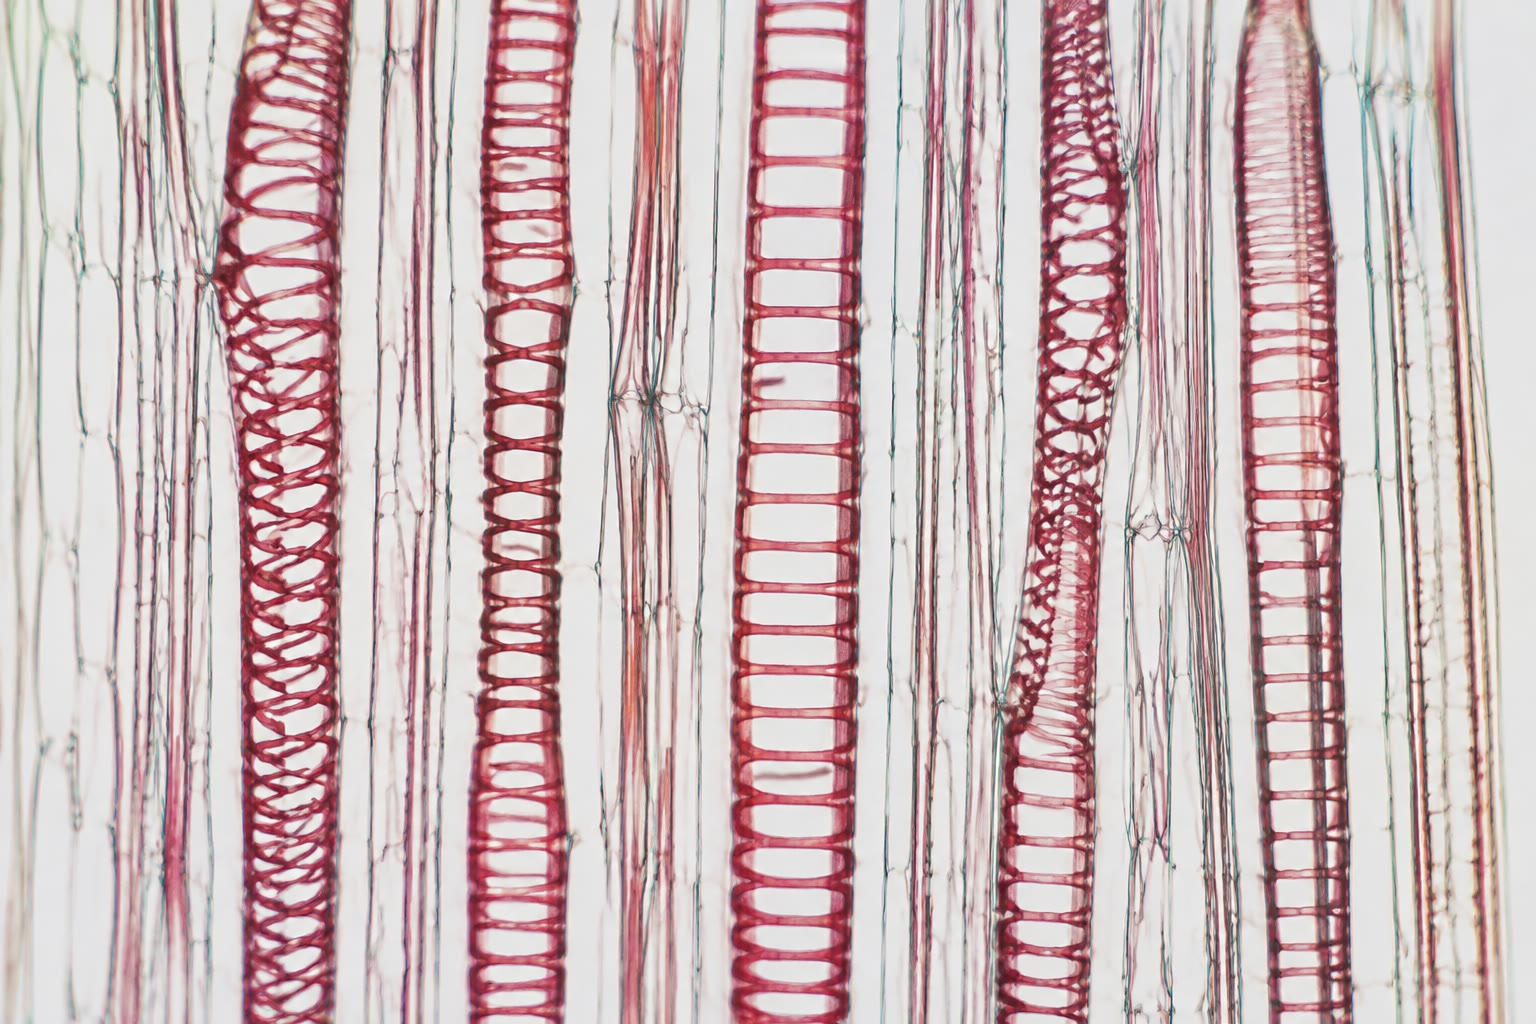
\includegraphics[width=0.52\linewidth]{images/book3/ai/b3-24-xylem-vessels.jpg}

{\small \omterm{def:b1:plant-transport:xylem}{Xyleemvaten} in de lengte doorgesneden: holle buizen waarvan de
wanden met ringen en spiralen van lignine zijn versterkt tegen de spanning
van het sap dat zij vervoeren.}
\end{omfigure}

\begin{omfigure}
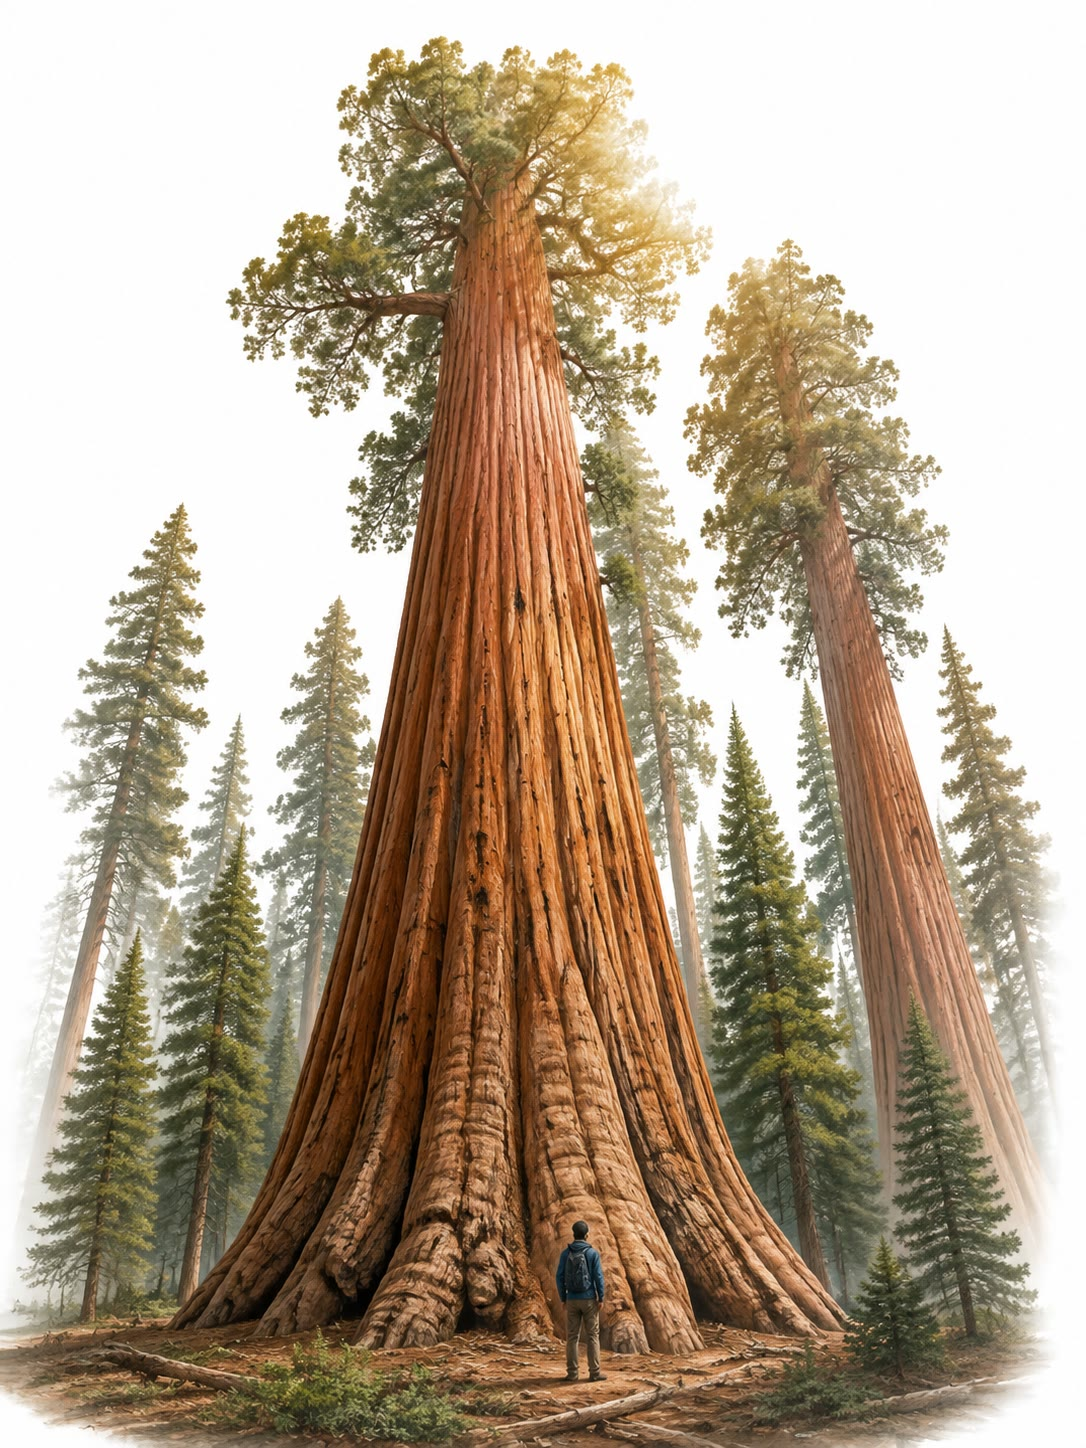
\includegraphics[width=0.36\linewidth]{images/book3/ai/b3-24-sequoia.jpg}

{\small Reuzensequoia's. Het sap bereikt hun kroon honderd meter hoog,
getrokken door de verdamping aan de \omterm{def:b1:flowering-plant-organization:organs}{bladeren} door waterkolommen onder een
spanning van twee megapascal of meer.}
\end{omfigure}

\begin{example}[De top van de boom]\label{ex:b1:plant-transport:top}
Op \qty{100}{m} vraagt het gewicht van de kolom alleen al \qty{1}{MPa}
spanning; de wrijving in de \omterm{def:b1:flowering-plant-organization:tissues}{vaten} doet daar overdag nog eens evenveel bij,
zodat het \omterm{def:b1:flowering-plant-organization:tissues}{xyleem} in de kroon dicht bij \qty{-2}{MPa} zit en de bladcellen,
om er water uit te trekken, nog lager: hun \omterm{def:b1:plant-transport:stoma}{huidmondjes} moeten eerder op de
dag sluiten en hun fotosynthese is trager dan die van een lage tak, en de
\omterm{def:b1:flowering-plant-organization:organs}{bladeren} bovenin zijn klein en dik. De hoogte van de hoogste bomen, zo'n
\qty{120}{m}, wordt vermoedelijk hierdoor bepaald: daarboven kunnen de
\omterm{def:b1:flowering-plant-organization:organs}{bladeren} de spanning niet houden zonder op een droge namiddag te caviteren.
\end{example}

\section{Suiker verplaatsen: drukstroming}

\begin{definition}[Floëem, zeefvaten, bron en put]\label{def:b1:plant-transport:phloem}
\index{floëem}\index{zeefvat}\index{bron}\index{put}
Suiker reist in het \emph{floëem}, in \emph{zeefvaten}: rijen levende
\omterm{def:b1:cell-unit-of-life:cell}{cellen} die hun kern en de meeste \omterm{def:b1:cell-unit-of-life:prokeuk}{organellen} hebben verloren maar hun
membranen behouden, met hun uiteinden aan elkaar gevoegd door geperforeerde
\emph{zeefplaten}, en elk verzorgd door een \emph{geleicel} die haar
\omterm{def:b1:proteins:peptide}{eiwitten} en \omterm{def:b1:water-small-molecules:atp}{ATP} levert. Het sap bevat \qtyrange{10}{30}{\%} sacharose, met
\omterm{def:b1:proteins:aminoacid}{aminozuren}, ionen en signaalmoleculen, en het stroomt van \emph{bronnen}
--- fotosynthetiserende \omterm{def:b1:flowering-plant-organization:organs}{bladeren}, of opslagorganen die worden geleegd ---
naar \emph{putten} --- groeitoppen, \omterm{def:b1:flowering-plant-organization:organs}{wortels}, vruchten, zaden, opslagorganen
die worden gevuld --- met \qtyrange{0.5}{1}{m/h}, in elke richting, en in
verschillende buizen in verschillende richtingen.
\end{definition}

\begin{theorem}[Drukstroming]\label{thm:b1:plant-transport:pressureflow}
\index{drukstroommechanisme}
Floëemsap beweegt door massastroming, gedreven door een verschil in
hydrostatische druk tussen bron en put (Münch, 1930). Bij de bron
\emph{laden} geleicellen sacharose tegen haar gradiënt in de \omterm{def:b1:plant-transport:phloem}{zeefvaten} (door
protonsymport, vanuit de \omterm{def:b1:plant-water-minerals:pathways}{apoplast}, of via plasmodesmata); de \omterm{def:b1:membranes-transport:osmosis}{waterpotentiaal}
van de buis daalt, er komt water uit het naburige \omterm{def:b1:flowering-plant-organization:tissues}{xyleem} binnen, en de
\omterm{def:b1:eukaryotic-cell:plantcell}{turgor} stijgt tot \qty{1}{MPa} of meer. Bij de put wordt de sacharose
\emph{ontladen} en verbruikt of opgeslagen, stijgt de \omterm{def:b1:membranes-transport:osmosis}{waterpotentiaal},
vertrekt er water, en is de \omterm{def:b1:eukaryotic-cell:plantcell}{turgor} laag. Daartussen stroomt het sap langs de
drukgradiënt door de zeefplaten, en neemt het mee wat erin is opgelost. De
plant besteedt alleen aan de twee uiteinden energie; de stroming zelf is
lijdelijk.
\end{theorem}
\begin{proof}[Bewijsmateriaal]
Een bladluis die op een \omterm{def:b1:flowering-plant-organization:organs}{stengel} zuigt steekt haar stilet in één enkel
\omterm{def:b1:plant-transport:phloem}{zeefvat}; snijd de luis weg en het achtergebleven stilet laat uren lang sap
lopen onder de eigen druk van de buis --- zuiver floëemsap, waarvan de
sacharoseconcentratie en de stroomsnelheid kunnen worden gemeten en waarvan
de druk, met een manometer op het stilet gemeten, ongeveer \qty{1}{MPa}
bedraagt bij een bron en lager richting de put. Gemerkt
$\mathrm{^{14}CO_2}$ dat aan een \omterm{def:b1:flowering-plant-organization:organs}{blad} wordt gevoerd verschijnt binnen
minuten in het \omterm{def:b1:plant-transport:phloem}{floëem} van de \omterm{def:b1:flowering-plant-organization:organs}{stengel} en beweegt met de snelheid die de
stiletstroom voorspelt; een stuk \omterm{def:b1:flowering-plant-organization:organs}{stengel} koelen, wat de levende \omterm{def:b1:cell-unit-of-life:cell}{cellen}
vertraagt maar een drukgedreven stroming nauwelijks raakt, vertraagt het
transport slechts weinig; het laden in het bronblad vergiftigen legt het
stil.
\end{proof}

\begin{omfigure}
\begin{tikzpicture}[font=\footnotesize, >=Stealth, line cap=round]
  % xylem and phloem tubes side by side
  \draw[line width=8pt, omDef!25] (1.0,0.3) -- (1.0,5.7); \node[anchor=south, omDef!70!black] at (1.0,5.8) {xyleem};
  \draw[line width=8pt, omExo!25] (3.6,0.3) -- (3.6,5.7); \node[anchor=south, omExo!70!black] at (3.6,5.8) {floëem (zeefvat)};
  % source at top
  \node[draw, thick, rounded corners=4pt, fill=omExo!15, align=center, minimum width=26mm] (src) at (7.2,5.0) {bron: blad\\ sacharose geladen};
  \node[draw, thick, rounded corners=4pt, fill=omProp!15, align=center, minimum width=26mm] (snk) at (7.2,1.0) {put: wortel, vrucht\\ sacharose ontladen};
  \draw[->, thick, omExo!70!black] (src.west) -- (3.9,5.0) node[midway, above, font=\scriptsize] {sacharose erin};
  \draw[->, thick, omProp!80!black] (3.3,1.0) -- (snk.west) node[midway, above, font=\scriptsize] {sacharose eruit};
  % water in from xylem at top, out to xylem at bottom
  \draw[->, thick, omDef!70!black] (1.3,4.6) -- (3.3,4.6) node[midway, below, font=\scriptsize] {water volgt};
  \draw[->, thick, omDef!70!black] (3.3,1.5) -- (1.3,1.5) node[midway, below, font=\scriptsize] {water keert terug};
  % flow arrows
  \draw[->, very thick, omExo!70!black] (3.6,4.2) -- (3.6,2.0) node[midway, right, align=left, font=\scriptsize] {massastroming langs\\ de drukgradiënt};
  \draw[->, very thick, omDef!70!black] (1.0,2.0) -- (1.0,4.2) node[midway, left, align=right, font=\scriptsize] {transpiratiestroom\\ (spanning)};
  \node[anchor=west, font=\scriptsize] at (3.9,5.5) {$\Psi_p \approx \qty{+1.0}{MPa}$};
  \node[anchor=west, font=\scriptsize] at (3.9,0.5) {$\Psi_p \approx \qty{+0.3}{MPa}$};
\end{tikzpicture}

{\small Drukstroming. Het laden van sacharose bij de bron trekt water uit
het \omterm{def:b1:flowering-plant-organization:tissues}{xyleem} naar binnen en verhoogt de druk; het ontladen bij de put laat
water naar buiten en verlaagt haar; het sap stroomt daartussen, en het water
keert via het \omterm{def:b1:flowering-plant-organization:tissues}{xyleem} terug.}
\end{omfigure}

\begin{omfigure}
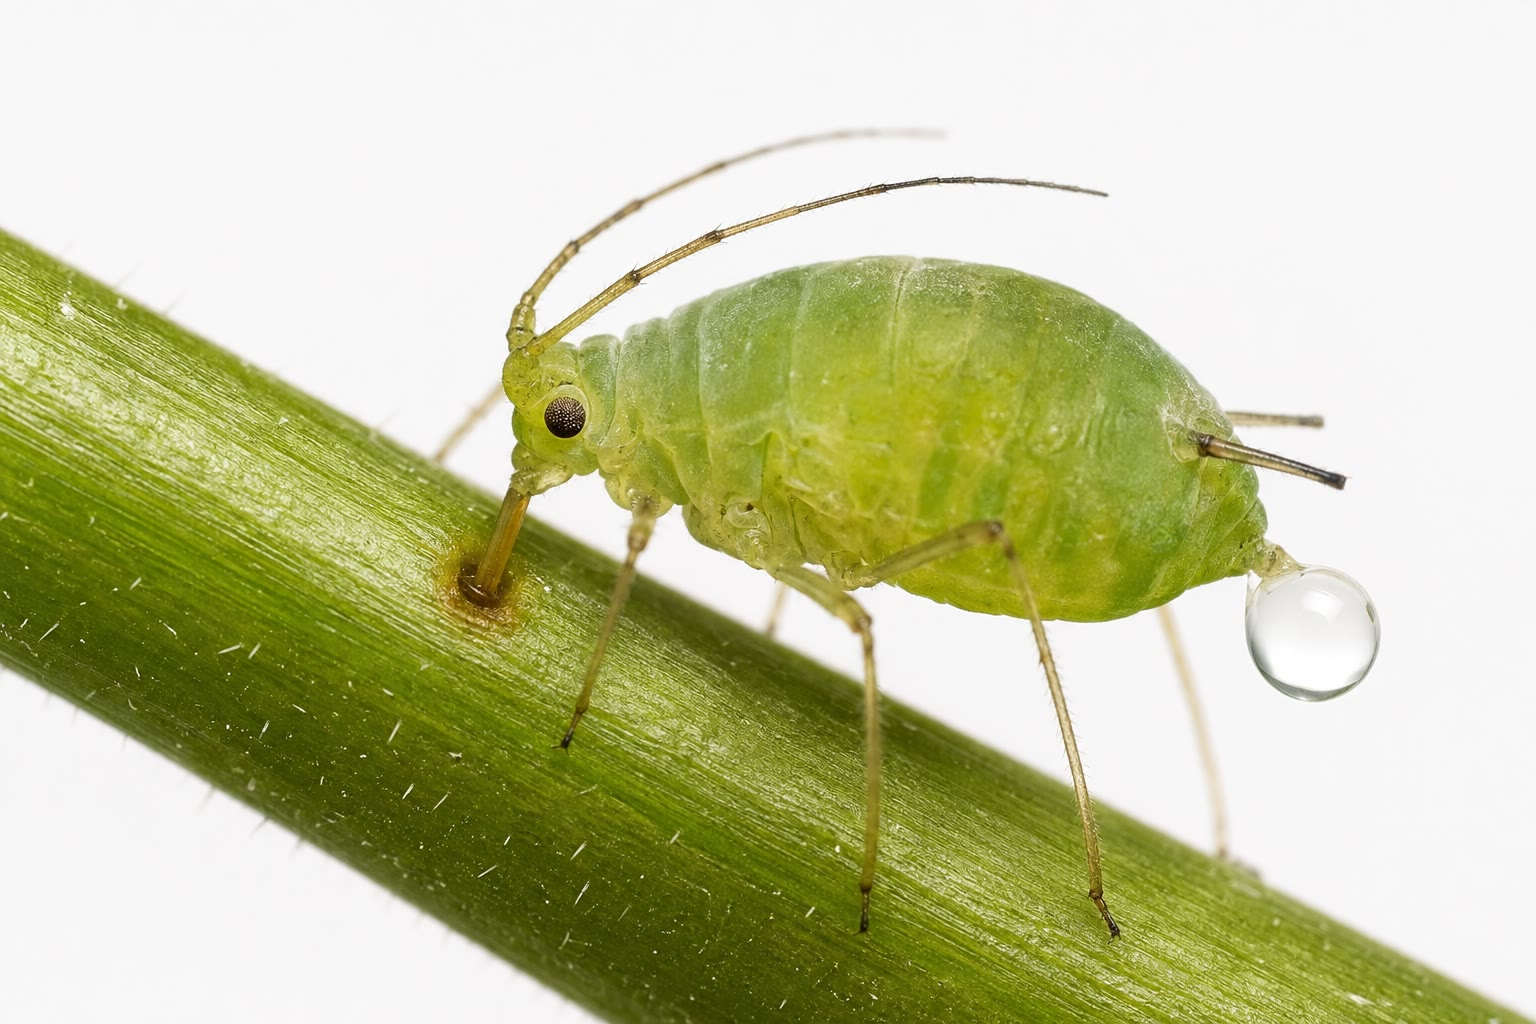
\includegraphics[width=0.5\linewidth]{images/book3/ai/b3-24-aphid-feeding.jpg}

{\small Een bladluis die op een \omterm{def:b1:flowering-plant-organization:organs}{stengel} zuigt: haar stilet, fijner dan een
haar, zit in één \omterm{def:b1:plant-transport:phloem}{zeefvat}, en de druk van het \omterm{def:b1:plant-transport:phloem}{floëem} drijft het sap het
insect in --- zoveel dat het overschot het als honingdauw verlaat.
Weggesneden wordt het stilet de kraan van de plantenfysioloog.}
\end{omfigure}

\begin{method}[Een transportproef lezen]\label{met:b1:plant-transport:translocation}
\begin{enumerate}
  \item Voer een \omterm{def:b1:flowering-plant-organization:organs}{blad} gemerkt $\mathrm{CO_2}$; bemonster de \omterm{def:b1:flowering-plant-organization:organs}{stengel}
        erboven en eronder met tussenpozen: de plaats van het merk tegen
        de tijd geeft de richting en de snelheid van de stroming.
  \item Ring de \omterm{def:b1:flowering-plant-organization:organs}{stengel} (verwijder een ring bast, die het \omterm{def:b1:plant-transport:phloem}{floëem} draagt,
        en laat het \omterm{def:b1:flowering-plant-organization:tissues}{xyleem} staan): boven de ring hoopt zich suiker op en
        eronder verhongeren de \omterm{def:b1:flowering-plant-organization:organs}{wortels} --- het \omterm{def:b1:plant-transport:phloem}{floëem} draagt haar, niet
        het \omterm{def:b1:flowering-plant-organization:tissues}{xyleem}; de boom sterft binnen een seizoen.
  \item Vang op twee hoogten sap op uit afgesneden bladluisstiletten: de
        daling van de sacharose en van de druk daartussen is de gradiënt
        die de stroming drijft.
  \item Verander de putten: haal de vruchten weg en het merk gaat naar de
        \omterm{def:b1:flowering-plant-organization:organs}{wortels}; zet het \omterm{def:b1:flowering-plant-organization:organs}{blad} in de schaduw en het wordt zelf een put. Het
        stroompatroon is het vraagpatroon.
\end{enumerate}
\end{method}

\begin{example}[Een aardappel in twee seizoenen]\label{ex:b1:plant-transport:potato}
In de zomer zijn de \omterm{def:b1:flowering-plant-organization:organs}{bladeren} bronnen en de knollen onder de grond de
putten: de sacharose stroomt omlaag, wordt ontladen, tot \omterm{def:b1:carbohydrates:polysaccharide}{zetmeel} omgezet, en
de knollen zwellen. In het voorjaar loopt de knol uit: haar \omterm{def:b1:carbohydrates:polysaccharide}{zetmeel} wordt
weer tot sacharose gemaakt, in het \omterm{def:b1:plant-transport:phloem}{floëem} geladen, en stroomt omhoog naar de
groeiende spruit --- dezelfde buis, de omgekeerde richting, omdat de bron en
de put van plaats zijn gewisseld.
\end{example}

\section{Het compromis}

\begin{proposition}[Watergebruiksefficiëntie]\label{prop:b1:plant-transport:wue}
\index{watergebruiksefficiëntie}
Elk \omterm{def:b1:plant-transport:stoma}{huidmondje} dat koolstofdioxide binnenlaat verliest water, en de ruil is
ongelijk: de binnenkant van het \omterm{def:b1:flowering-plant-organization:organs}{blad} is met damp verzadigd en de lucht
buiten is droog, terwijl $\mathrm{CO_2}$ buiten op \qty{0.04}{\%} staat en
binnen lager, zodat de gradiënt van water naar buiten honderden keren de
gradiënt van koolstofdioxide naar binnen is. Een C3-blad verliest
\qtyrange{200}{500}{} watermoleculen per vastgelegde $\mathrm{CO_2}$; een
C4-blad, dat $\mathrm{CO_2}$ concentreert en zijn \omterm{def:b1:plant-transport:stoma}{huidmondjes} nauwer houdt,
\qtyrange{100}{200}{}; een \omterm{def:b1:photosynthesis:c4cam}{CAM-plant}, die alleen 's nachts opent,
\qtyrange{20}{50}{} (\cref{ch:b1:photosynthesis}). De
\emph{\omterm{prop:b1:plant-transport:wue}{watergebruiksefficiëntie}} is de gewonnen koolstof per verloren water,
en de verbetering ervan --- door midden op de dag te sluiten, door verzonken
\omterm{def:b1:plant-transport:stoma}{huidmondjes} en dikke \omterm{def:b1:flowering-plant-organization:tissues}{cuticula}'s, door de C4- en de CAM-weg --- is het
aandeel van de plant in de afspraak met een droge dampkring.
\end{proposition}

\begin{example}[De afspraak in getallen]\label{ex:b1:plant-transport:bargain}
Een maïsplant die anderhalve liter per dag verdampt legt zo'n \qty{10}{g}
koolstofdioxide vast: \qty{80}{mol} water voor \qty{0.23}{mol}
$\mathrm{CO_2}$, driehonderdvijftig tegen één. Een tarweveld verdampt in
één seizoen vijfhonderd ton water per hectare om acht ton graan te maken;
het water is de prijs van de koolstof, en op de meeste akkers ter wereld is
het de prijs die de oogst begrenst.
\end{example}

\section{Opgaven}

\begin{exercise}[$\star$]\label{exo:b1:plant-transport:1}
Leg uit hoe de vorm en de wanden van \omterm{def:b1:plant-transport:stoma}{sluitcellen} een stijging van de \omterm{def:b1:eukaryotic-cell:plantcell}{turgor}
in een open porie omzetten.
\end{exercise}

\begin{exercise}[$\star$]\label{exo:b1:plant-transport:2}
Formuleer het cohesie--spanningsmechanisme in drie zinnen: waar de kracht
vandaan komt, wat haar doorgeeft, en wat zij bij de \omterm{def:b1:flowering-plant-organization:organs}{wortel} doet.
\end{exercise}

\begin{exercise}[$\star$]\label{exo:b1:plant-transport:3}
Op welk uur is de \omterm{thm:b1:plant-transport:cohesiontension}{transpiratie} volgens de dagfiguur het hoogst, wanneer
bereikt de \omterm{def:b1:membranes-transport:osmosis}{waterpotentiaal} van het \omterm{def:b1:flowering-plant-organization:organs}{blad} haar minimum, en waarom sluiten de
\omterm{def:b1:plant-transport:stoma}{huidmondjes} zich midden op de dag deels?
\end{exercise}

\begin{exercise}[$\star$]\label{exo:b1:plant-transport:4}
Omschrijf bron en put, en zeg wat er bij elk gebeurt in het
\omterm{thm:b1:plant-transport:pressureflow}{drukstroommechanisme}.
\end{exercise}

\begin{exercise}[$\star\star$]\label{exo:b1:plant-transport:5}
Bereken de spanning die nodig is om een waterkolom van \qty{30}{m} hoog te
houden ($\rho g h$), en het totaal als de wrijving die verdubbelt. Wat moet
de \omterm{def:b1:membranes-transport:osmosis}{waterpotentiaal} van de \omterm{def:b1:flowering-plant-organization:organs}{bladeren} op die hoogte ten minste zijn?
\end{exercise}

\begin{exercise}[$\star\star$]\label{exo:b1:plant-transport:6}
De stroming door een buis schaalt als $r^4$. Vergelijk de stroming door één
vat met een straal van \qty{100}{\micro m} met die door het aantal
\omterm{def:b1:plant-transport:xylem}{tracheïden} van \qty{10}{\micro m} met dezelfde totale doorsnede. Waarom
houden planten de nauwe?
\end{exercise}

\begin{exercise}[$\star\star$]\label{exo:b1:plant-transport:7}
Floëemsap met \qty{20}{\%} sacharose (\qty{0.6}{mol/L}) heeft een
\omterm{def:b1:membranes-transport:osmosis}{osmotische potentiaal} van ongeveer \qty{-1.5}{MPa}. Welke \omterm{def:b1:eukaryotic-cell:plantcell}{turgor} bereikt het
\omterm{def:b1:plant-transport:phloem}{zeefvat} in evenwicht naast een \omterm{def:b1:flowering-plant-organization:tissues}{xyleem} op \qty{-0.5}{MPa}? En bij een put
waar het sap \qty{5}{\%} sacharose bevat ($\Psi_s = \qty{-0.4}{MPa}$) naast
hetzelfde \omterm{def:b1:flowering-plant-organization:tissues}{xyleem}? Welk drukverschil drijft de stroming?
\end{exercise}

\begin{exercise}[$\star\star$]\label{exo:b1:plant-transport:8}
Een bladluisstilet laat \qty{1}{\micro L} per uur sap lopen met
\qty{20}{\%} sacharose. Bereken, als het \omterm{def:b1:plant-transport:phloem}{zeefvat} een straal van
\qty{10}{\micro m} heeft, de snelheid van het sap en de suiker die per uur
wordt afgeleverd.
\end{exercise}

\begin{exercise}[$\star\star$]\label{exo:b1:plant-transport:9}
Leg uit waarom het ringen van een boom hem binnen een seizoen doodt, terwijl
zijn \omterm{def:b1:flowering-plant-organization:organs}{bladeren} na het snijden van de ring nog wekenlang groen blijven.
\end{exercise}

\begin{exercise}[$\star\star\star$]\label{exo:b1:plant-transport:10}
De luchtholten van een \omterm{def:b1:flowering-plant-organization:organs}{blad} zijn bij \qty{25}{\celsius} verzadigd
(\qty{23}{g/m^3} damp); de buitenlucht bevat \qty{9}{g/m^3}.
$\mathrm{CO_2}$ staat buiten op \qty{0.72}{g/m^3} en binnen op
\qty{0.45}{g/m^3}. De twee gassen diffunderen door dezelfde poriën, waarbij
water 1,6 keer sneller diffundeert dan $\mathrm{CO_2}$. Bereken de
verhouding van verloren water tot gewonnen $\mathrm{CO_2}$, naar massa en
per molecuul.
\end{exercise}

\begin{exercise}[$\star\star\star$]\label{exo:b1:plant-transport:11}
Op een hete droge namiddag caviteert een vat. Beschrijf wat er met de
waterkolom, met de spanning in de naburige \omterm{def:b1:flowering-plant-organization:tissues}{vaten} en met het \omterm{def:b1:flowering-plant-organization:organs}{blad} dat het
voedde gebeurt; leg uit hoe stippels de schade beperken en hoe de plant zich
in de nacht of in de lente herstelt.
\end{exercise}

\begin{exercise}[$\star\star\star$]\label{exo:b1:plant-transport:12}
``Een boom is een lont tussen de bodem en de hemel, met een suikerpijp die
de andere kant op loopt.'' Bespreek dat in een alinea: wat elk stelsel
vervoert, wat het drijft, waar de plant energie besteedt, en waar zij er
geen besteedt.
\end{exercise}

\section{Vraagstuk: de sequoia}

\begin{problem}[{Weekendvraagstuk --- een boom van honderd meter op een
zomerdag: de spanning in zijn kroon, de snelheid van het sap, het water dat
hij verplaatst, de suiker die hij omlaag stuurt en de koolstof die hij
daarmee koopt, eindigend op de xyleemspanning in de kroon}]
\label{pb:b1:plant-transport:1}
Een sequoia is \qty{100}{m} hoog met een kroon van \qty{2000}{m^2} \omterm{def:b1:flowering-plant-organization:organs}{blad}. Op
een zomerdag verdampt hij \qty{600}{L} water in \qty{12}{h} door spinthout
met een doorsnede van \qty{0.5}{m^2}, waarvan \qty{20}{\%} geleidend lumen
is. Water: $\rho = \qty{1000}{kg/m^3}$, $g =
\qty{9.8}{m/s^2}$, \qty{18}{g/mol}. De wrijving langs de stam kost evenveel
spanning als de zwaartekracht. \omterm{def:b1:membranes-transport:osmosis}{Waterpotentiaal} van de bodem
\qty{-0.1}{MPa}. De kroon legt \qty{4}{\micro mol} $\mathrm{CO_2}$ per
vierkante meter \omterm{def:b1:flowering-plant-organization:organs}{blad} per seconde vast gedurende \qty{12}{h}; sacharose weegt
\qty{342}{g/mol} en draagt twaalf koolstofatomen; het floëemsap bevat naar
massa \qty{15}{\%} sacharose (dichtheid \qty{1.06}{g/mL}) en stroomt met
\qty{0.6}{m/h}.

\medskip
\noindent\textbf{Deel I --- Spanning.}
\begin{enumerate}
  \item Bereken de spanning die nodig is om de kolom tegen de
        zwaartekracht in te dragen.
  \item Tel de wrijving erbij: hoe groot is de xyleemspanning in de
        kroon?
  \item Bereken de \omterm{def:b1:membranes-transport:osmosis}{waterpotentiaal} van het \omterm{def:b1:flowering-plant-organization:tissues}{xyleem} in de kroon, met
        $\Psi_s = 0$ voor het sap.
  \item Hoe groot moet de \omterm{def:b1:membranes-transport:osmosis}{waterpotentiaal} van de bladcellen in de kroon
        zijn opdat er water binnenkomt? Welke \omterm{def:b1:eukaryotic-cell:plantcell}{turgor} hebben zij als hun
        $\Psi_s = \qty{-2.5}{MPa}$?
  \item Vergelijk dat met een \omterm{def:b1:flowering-plant-organization:organs}{blad} op \qty{10}{m} in dezelfde boom ($\Psi_s =
        \qty{-1.5}{MPa}$).
  \item Water in fijne buizen verdraagt ongeveer \qty{-30}{MPa}; waarom
        groeit de boom dan niet eenvoudig tot \qty{1000}{m}?
\end{enumerate}

\medskip
\noindent\textbf{Deel II --- Stroming.}
\begin{enumerate}[resume]
  \item Bereken de transpiratiesnelheid in liters per uur en in kubieke
        meters per seconde.
  \item Bereken de geleidende doorsnede van het spinthout.
  \item Bereken de gemiddelde snelheid van het sap.
  \item Bereken de massa water in het geleidende lumen van de stam
        (\qty{100}{m} daarvan).
  \item Hoe lang doet een watermolecuul er bij die snelheid over om van
        \omterm{def:b1:flowering-plant-organization:organs}{wortel} naar kroon te reizen?
  \item Bereken de \omterm{thm:b1:plant-transport:cohesiontension}{transpiratie} per vierkante meter \omterm{def:b1:flowering-plant-organization:organs}{blad} per uur, in
        grammen, en per seconde in millimol.
  \item Het sap stroomt over \qty{100}{m} langs een potentiaalgradiënt
        van \qty{-0.1}{} bij de bodem tot de waarde van de kroon uit vraag
        3. Hoe groot is de gradiënt in megapascal per meter? Hoe
        verhoudt die zich tot het aandeel van de zwaartekracht alleen?
\end{enumerate}

\medskip
\noindent\textbf{Deel III --- Suiker.}
\begin{enumerate}[resume]
  \item Bereken de $\mathrm{CO_2}$ die de kroon per dag vastlegt, in
        mol.
  \item Bereken de sacharose die daarmee overeenkomt, in mol en in
        kilogram.
  \item De helft wordt in de kroon verademd; de rest gaat het \omterm{def:b1:plant-transport:phloem}{floëem} in
        omlaag. Bereken de massa sacharose die per dag wordt vervoerd en
        de massa sap die haar draagt.
  \item Bereken het volume sap en, bij \qty{0.6}{m/h}, de doorsnede aan
        \omterm{def:b1:plant-transport:phloem}{zeefvaten} die nodig is om het in \qty{24}{h} te vervoeren.
  \item Bereken de tijd die sacharose van kroon naar \omterm{def:b1:flowering-plant-organization:organs}{wortel} doet.
  \item Bereken de watergebruiksverhouding: mol verdampt water per mol
        vastgelegde $\mathrm{CO_2}$.
\end{enumerate}

\medskip
\noindent\textbf{Deel IV --- Compromissen.}
\begin{enumerate}[resume]
  \item De \omterm{def:b1:membranes-transport:osmosis}{waterpotentiaal} van het floëemsap in de kroon, met
        $\Psi_s = \qty{-1.2}{MPa}$ en \omterm{def:b1:eukaryotic-cell:plantcell}{turgor} \qty{1.0}{MPa}: bereken die
        en vergelijk haar met die van het \omterm{def:b1:flowering-plant-organization:tissues}{xyleem} daar. Welke kant beweegt
        het water tussen beide op, en strookt dat met het laden?
  \item Bij de \omterm{def:b1:flowering-plant-organization:organs}{wortel} bevat het floëemsap \qty{5}{\%} sacharose ($\Psi_s =
        \qty{-0.4}{MPa}$) en staat het \omterm{def:b1:flowering-plant-organization:tissues}{xyleem} op \qty{-0.3}{MPa}. Bij
        welke \omterm{def:b1:eukaryotic-cell:plantcell}{turgor} is de $\Psi$ van het \omterm{def:b1:plant-transport:phloem}{floëem} gelijk aan die van het
        \omterm{def:b1:flowering-plant-organization:tissues}{xyleem}? Welk drukverschil tussen kroon en \omterm{def:b1:flowering-plant-organization:organs}{wortel} drijft de
        stroming?
  \item De \omterm{def:b1:plant-transport:stoma}{huidmondjes} sluiten midden op de dag en de \omterm{thm:b1:plant-transport:cohesiontension}{transpiratie}
        halveert. Bereken de wrijvingsspanning en de xyleempotentiaal in
        de kroon opnieuw. Wat wint en wat verliest de boom?
  \item In een droog jaar zakt de bodem naar \qty{-1.0}{MPa}. Bereken de
        kroonpotentiaal opnieuw bij volle \omterm{thm:b1:plant-transport:cohesiontension}{transpiratie}. Kunnen de
        kroonbladeren ($\Psi_s = \qty{-2.5}{MPa}$) nog enige \omterm{def:b1:eukaryotic-cell:plantcell}{turgor}
        houden? Wat moet de boom doen?
  \item Leg uit waarom de hoogste \omterm{def:b1:flowering-plant-organization:organs}{bladeren} de kleinste en dikste zijn.
  \item Geef het resultaat: de xyleemspanning in de kroon van een boom van
        \qty{100}{m} op een zomerdag, en de sapsnelheid die daarbij hoort.
\end{enumerate}
\end{problem}
